\section{Opgave 1}
Opgave et går ud på at lave et program, der begregner summen af kvadratrødderne fra 0 til N; altså:
\begin{center}
$\displaystyle\sum_{i=0}^{N} \sqrt{i}$
\end{center}
Derudover skal vi gøre brug af flere tråde, så X antal tråde hver står for en X'ende del af beregningerne. Vi har allerede fået udleveret kode, der kan beregne:

\begin{center}
$\displaystyle\sum_{i=0}^{N} i$,
\end{center}
så det eneste vi skal gøre er at:

\begin{itemize}
\item Dele beregningerne op, så hver tråd får en X'ende del af beregningerne at udføre.
\item Modificere selve beregningen af summen, så det er $\sqrt{i}$ og ikke i, der bliver beregnet.
\end{itemize}

\subsection{Divide and conquer}
For at gøre beregningerne opdelelige, så flere tråde kan arbejde sammen om dem, har vi først lavet en struct kaldt ThreadData. Den indeholder tre felter:
\begin{description}
\item[lower] er værdien, en tråd skal summere fra.
\item[upper] er værdien, en tråd skal summere til.
\item[partialSum] er summen af kvadratrødderne fra \textbf{lower} til \textbf{upper}. 
\end{description}

I starten beregnes tallet sumSegment, der er N divideret med antallet af tråde. Så laves det antal tråde, der er blevet specificeret og samme antal ThreadData structs, hvor deres \textbf{lower} bliver sat til sumSegment gange det nummer, som tråden er plus et. Derefter bliver deres \textbf{upper} sat til sumSegment gange det nummer, som tråden er, plus sumSegment. Det gør, at alle tråde får en lige stor andel af beregningerne, når \begin{verbatim}pthread_create()\end{verbatim} bliver kaldt med en ThreadData som parameter. 

\subsection{Fra i til $\sqrt{i}$}
Inde i runner() kører et forloop, der sætter partialSum for den tilhørende ThreadData til summen af alle kvadratrødder i intervallet \textbf{lower} til \textbf{upper}. Tilbage i main metoden summere alle ThreadData's partialSum, og resultatet printes ud.

\subsection{Resultater}
Programmet solution blev kørt med N som 1.000.000.000. Tabellen herunder viser hvor lang tid beregningerne tog med forskellige antal tråde.

\begin{center}
  \begin{tabular}{ | l | c | r | }
    \hline
    \textbf{Number of threads:} & \textbf{Real-time:} \\ \hline
    1 & 5.090 \\ \hline
	2 & 3.271 \\ \hline
	3 & 2.360 \\ \hline
	4 & 2.454 \\ \hline
	5 & 2.250 \\ \hline
	6 & 2.120 \\ \hline
	7 & 2.169 \\ \hline
	8 & 2.134 \\ \hline
	16 & 1.881 \\ \hline
	32 & 1.828 \\ \hline
  \end{tabular}
\end{center}

\begin{figure}[h!]
  \caption{Speed-up graf}
  \centering
    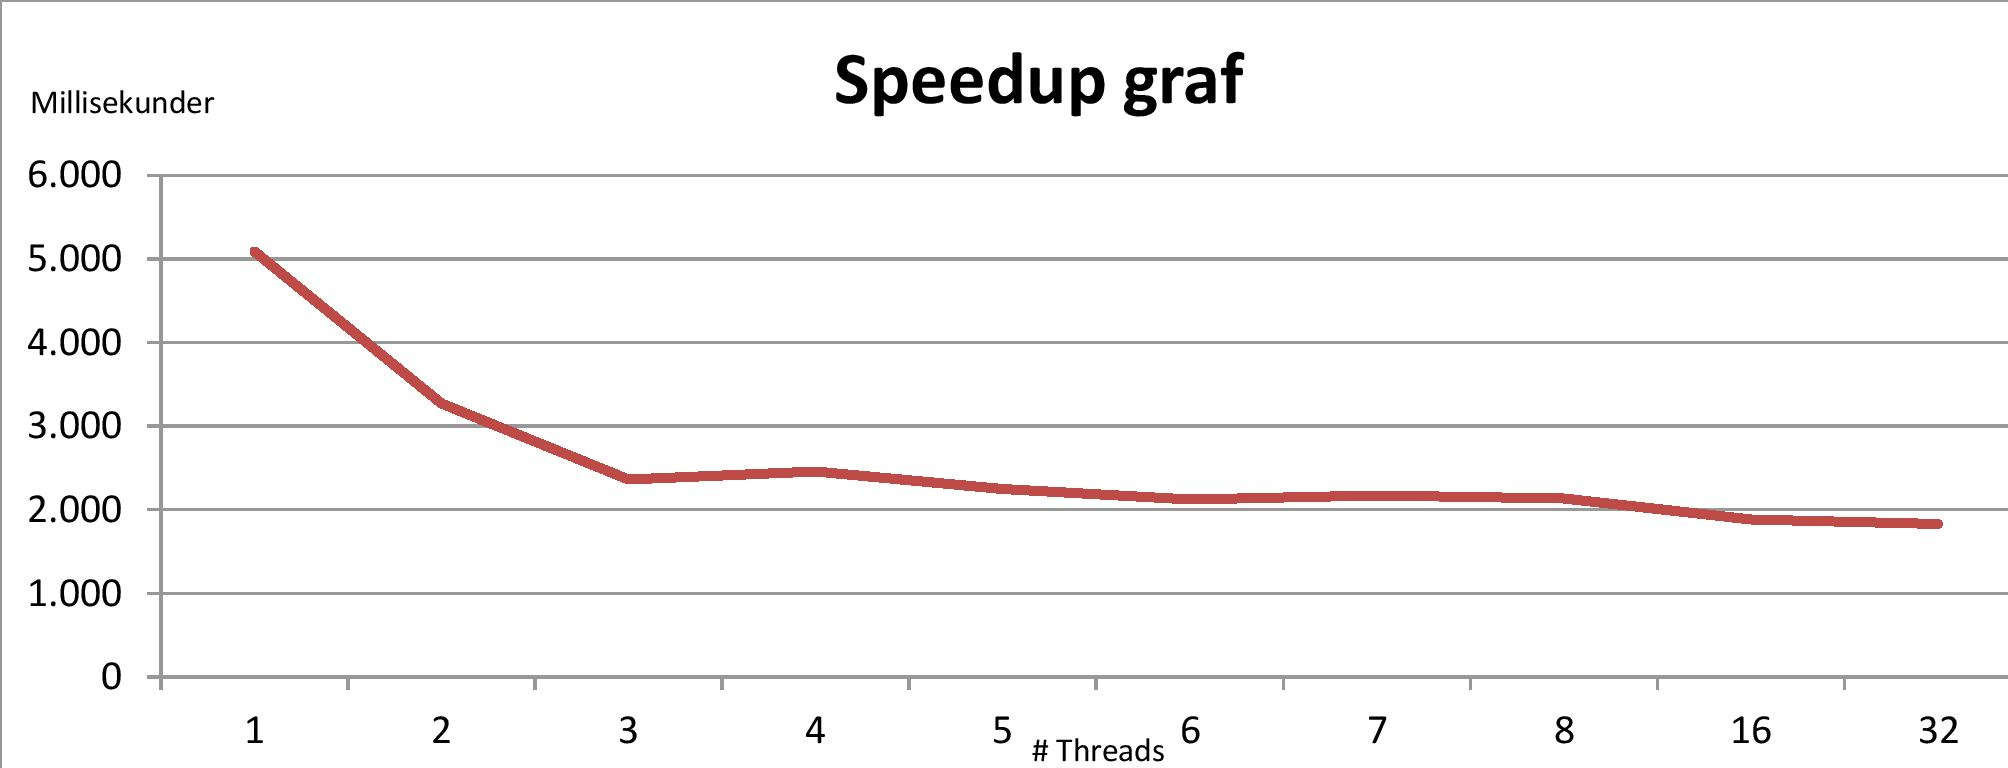
\includegraphics[width=0.9\textwidth]{Speedup-graf}
\end{figure}
